\documentclass{article}

% NeurIPS 2025 style. "preprint" reveals author names and drops the anonymous
% submission notice -- appropriate for a course project (not an anonymous review).
\usepackage[preprint]{neurips_2025}

\usepackage[utf8]{inputenc}
\usepackage[T1]{fontenc}
\usepackage{hyperref}
\usepackage{url}
\usepackage{booktabs}
\usepackage{amsfonts}
\usepackage{amsmath}
\usepackage{amssymb}
\usepackage{nicefrac}
\usepackage{microtype}
\usepackage{graphicx}
\usepackage{subcaption}
\usepackage{multirow}
\usepackage{xcolor}
\usepackage{pifont}   % \ding{55} cross mark in the ablation table
\usepackage{listings}

\graphicspath{{figures/}}

% ---- code listing style for the "code snippets" rubric item ----
\definecolor{codegreen}{rgb}{0.0,0.5,0.0}
\definecolor{codegray}{rgb}{0.5,0.5,0.5}
\definecolor{codepurple}{rgb}{0.58,0.0,0.82}
\definecolor{backcolour}{rgb}{0.96,0.96,0.94}
\lstdefinestyle{py}{
  backgroundcolor=\color{backcolour},
  commentstyle=\color{codegreen},
  keywordstyle=\color{blue},
  numberstyle=\tiny\color{codegray},
  stringstyle=\color{codepurple},
  basicstyle=\ttfamily\scriptsize,
  breakatwhitespace=false, breaklines=true, captionpos=b,
  keepspaces=true, numbers=left, numbersep=5pt,
  showspaces=false, showstringspaces=false, showtabs=false,
  tabsize=2, language=Python, frame=single, framesep=4pt
}
\lstset{style=py}

\title{Residual Multi-Head Mixing GAT:\\
A Skip-Connected Attention Model for Node Classification on Cora}

\author{%
  \textbf{Group 03} \\
  Hanoi University of Science and Technology \\
  \texttt{minhdotpc@gmail.com} \\
  \AND
  Do Tuan Minh (20261057M) \quad Hoang Huy Chien (20261069M) \quad
  Tran Tien Dung (20252574M) \\
  Tran Manh Tien (20252762M) \quad Nguyen Tien Duc (20252076M)
}

\begin{document}

\maketitle

\begin{abstract}
Node classification on citation networks is a canonical semi-supervised learning
task in which only a handful of labelled nodes must propagate information across a
large graph. We study this problem on the \textbf{Cora} dataset and present a
systematic comparison between a feature-only Multi-Layer Perceptron (MLP) baseline
and four graph neural networks: Graph Convolutional Network (GCN), GraphSAGE, Graph
Attention Network (GAT), and a proposed \textbf{Residual Multi-Head Mixing GAT}.
The proposed model augments a two-layer multi-head attention backbone with a linear
skip connection from the raw input features to the output logits, and an optional
DropEdge regularizer. Across five random seeds, the proposed model reaches
$83.34\% \pm 0.71\%$ test accuracy, outperforming vanilla GAT ($82.72\%$), GCN
($82.76\%$), and GraphSAGE ($81.30\%$), while all graph models improve over the MLP
baseline ($58.88\%$) by roughly 24 absolute points. A controlled ablation isolates
each design choice and shows that the residual skip is the dominant contributor
($+1.7\%$), whereas DropEdge is neutral on a graph as small as Cora. We release the
full code, configuration, and reproduction notebook.
\end{abstract}

% =====================================================================
\section{Introduction}
\label{sec:intro}

Graphs are a natural representation for relational data: social networks, molecules,
knowledge bases, and---in this work---\emph{citation networks}, where nodes are
scientific papers and edges are citations. A recurring task on such data is
\textbf{node classification}: given the features of every node but the labels of
only a small subset, predict the labels of the remaining nodes. Because labels are
scarce and the unlabelled nodes are visible at training time, this is a
\emph{transductive, semi-supervised} problem, and the graph structure is precisely
what allows label information to travel from the few labelled seeds to the rest of
the network~\cite{yang2016planetoid,sen2008collective}.

\paragraph{Why the graph matters.}
A model that ignores the edges and classifies each paper from its bag-of-words
features alone throws away the single most informative signal: papers cite papers on
the same topic. Our first empirical result quantifies exactly this---an MLP that sees
only node features reaches $58.9\%$ accuracy, while the simplest graph model in our
study jumps to $82.8\%$. The $\sim$24-point gap is the motivation for the entire
project: \emph{how should structure be incorporated, and which architectural choices
matter?}

\paragraph{From convolution to attention.}
Graph Convolutional Networks~\cite{kipf2017gcn} aggregate neighbour features with
fixed, degree-normalized weights. GraphSAGE~\cite{hamilton2017graphsage} generalizes
aggregation to learnable functions and inductive settings. Graph Attention
Networks~\cite{velickovic2018gat} instead \emph{learn} how much each neighbour should
contribute through a multi-head attention mechanism. A well-known failure mode of
deep message passing is \textbf{over-smoothing}: after several rounds of aggregation,
node representations converge and become indistinguishable~\cite{li2018deeper,
oono2020oversmoothing}. Residual/skip connections~\cite{he2016resnet,xu2018jknet} and
edge-dropping regularizers~\cite{rong2020dropedge} are two standard remedies.

\paragraph{Contributions.}
This report makes the following contributions.
\begin{enumerate}
  \item A clean, reproducible benchmark of MLP, GCN, GraphSAGE and GAT on Cora under
        an identical training protocol and five-seed evaluation
        (Section~\ref{sec:results}).
  \item A proposed \textbf{Residual Multi-Head Mixing GAT} that adds a raw-feature
        skip connection $H_0 W_{\text{skip}}$ and optional DropEdge to a two-layer
        GAT (Section~\ref{sec:proposed}), achieving the best accuracy in our study.
  \item A controlled \textbf{ablation} that separates the effect of the residual
        skip, DropEdge, and the number of attention heads
        (Section~\ref{sec:ablation}), together with a discussion of when each
        technique helps (Section~\ref{sec:discussion}).
\end{enumerate}

The remainder of the paper is organized as follows.
Section~\ref{sec:problem} formalizes the task and describes the dataset.
Section~\ref{sec:methods} details every model.
Section~\ref{sec:setup} gives the experimental protocol.
Sections~\ref{sec:results} and~\ref{sec:ablation} report results and the ablation.
Sections~\ref{sec:discussion} and~\ref{sec:limitations} discuss findings and
limitations, and Section~\ref{sec:conclusion} concludes.

% =====================================================================
\section{Problem Formulation and Dataset}
\label{sec:problem}

\subsection{Task definition}
Let $G = (V, E)$ be an undirected graph with $N = |V|$ nodes. Each node $v$ has a
feature vector $x_v \in \mathbb{R}^{F}$ stacked into a matrix
$X \in \mathbb{R}^{N \times F}$, and a label $y_v \in \{1,\dots,C\}$. We are given the
labels of a small training set $V_{\text{train}} \subset V$ and must predict the
labels of the remaining nodes. A model $f_\theta$ produces class scores
$Z = f_\theta(X, A) \in \mathbb{R}^{N \times C}$, where $A \in \{0,1\}^{N \times N}$
is the adjacency matrix, and is trained by minimizing the cross-entropy over the
labelled nodes:
\begin{equation}
  \mathcal{L}(\theta) = -\frac{1}{|V_{\text{train}}|}
  \sum_{v \in V_{\text{train}}} \log \frac{\exp(Z_{v,y_v})}{\sum_{c=1}^{C}\exp(Z_{v,c})}.
  \label{eq:loss}
\end{equation}
Because the whole graph (including test nodes' features and edges) is available
during training, the setting is \emph{transductive}.

\subsection{The Cora dataset}
Cora~\cite{sen2008collective,yang2016planetoid} is a citation network of machine
learning papers. Each node is a paper described by a $1433$-dimensional binary
bag-of-words vector (presence/absence of dictionary words); each undirected edge is a
citation; each paper belongs to one of $C=7$ topics (e.g.\ \emph{Neural Networks},
\emph{Reinforcement Learning}, \emph{Probabilistic Methods}). We use the standard
public (``Planetoid'') split loaded through PyTorch Geometric~\cite{fey2019pyg}. Its
statistics are summarized in Table~\ref{tab:dataset}.

\begin{table}[h]
  \centering
  \caption{Cora dataset statistics (standard public split).}
  \label{tab:dataset}
  \begin{tabular}{lr}
    \toprule
    Property & Value \\
    \midrule
    Nodes (papers)            & 2{,}708 \\
    Edges (citations)         & 10{,}556 \\
    Features per node         & 1{,}433 \\
    Classes (topics)          & 7 \\
    Training nodes            & 140 (20 per class) \\
    Validation nodes          & 500 \\
    Test nodes                & 1{,}000 \\
    Label rate ($|V_{\text{train}}|/N$) & 5.2\% \\
    \bottomrule
  \end{tabular}
\end{table}

Two properties make Cora a demanding but instructive benchmark. First, the
\textbf{label rate is very low} ($5.2\%$)---only 140 labelled nodes must classify
2{,}708. Second, the features are \textbf{sparse and high-dimensional}, so a purely
feature-based classifier struggles to separate classes without the relational signal.

\paragraph{Structure and homophily.} Cora is strongly \emph{homophilous}: citations
overwhelmingly connect papers of the same topic, so a node's label is well predicted by
its neighbours' labels. With $10{,}556$ edges over $2{,}708$ nodes the average degree is
$\approx 3.9$, i.e.\ the graph is sparse, and it contains a small number of disconnected
components. These two facts jointly explain much of what we observe later: homophily is
why even the simplest neighbour-averaging model (GCN) is extremely strong, and sparsity
is why aggressive edge removal (DropEdge) has little room to help---there are few
redundant edges to drop. They also caution against over-generalizing: on
\emph{heterophilous} graphs, where neighbours often disagree, the ranking of these
models can invert.

\subsection{Notation}
Table~\ref{tab:notation} collects the symbols used throughout. We write $H^{(l)}$ for
the node-representation matrix at layer $l$ (with $H^{(0)} = X$), $\mathcal{N}(v)$ for
the one-hop neighbourhood of node $v$, and $\sigma(\cdot)$ for a pointwise
nonlinearity.

\begin{table}[h]
  \centering
  \caption{Notation used throughout the paper.}
  \label{tab:notation}
  \begin{tabular}{ll@{\hskip 3em}ll}
    \toprule
    Symbol & Meaning & Symbol & Meaning \\
    \midrule
    $G=(V,E)$ & graph, nodes, edges      & $N$ & number of nodes ($2{,}708$) \\
    $X \in \mathbb{R}^{N\times F}$ & node features & $F$ & feature dim ($1{,}433$) \\
    $A$ & adjacency matrix              & $C$ & number of classes ($7$) \\
    $\tilde{A}=A+I$ & self-looped adj.   & $\tilde{D}$ & degree matrix of $\tilde{A}$ \\
    $H^{(l)}$ & layer-$l$ features       & $\mathcal{N}(v)$ & neighbours of $v$ \\
    $W^{(l)}$ & layer-$l$ weights        & $K$ & number of attention heads \\
    $\alpha_{vu}$ & attention weight     & $Z$ & output logits $\in\mathbb{R}^{N\times C}$ \\
    \bottomrule
  \end{tabular}
\end{table}

% =====================================================================
\section{Background: The Message-Passing Framework}
\label{sec:background}

All four graph models in this study are instances of a single \emph{message-passing}
template~\cite{kipf2017gcn,hamilton2017graphsage,velickovic2018gat}. Each layer updates
every node by (i)~\textbf{aggregating} transformed messages from its neighbours and
(ii)~\textbf{combining} the aggregate with the node's own state:
\begin{equation}
  m_v^{(l)} = \textsc{Aggregate}\Big(\big\{\, \phi(h_u^{(l)}) : u \in \mathcal{N}(v) \,\big\}\Big),
  \qquad
  h_v^{(l+1)} = \textsc{Update}\Big(h_v^{(l)},\, m_v^{(l)}\Big).
  \label{eq:mpnn}
\end{equation}
The models differ only in \emph{how} they instantiate \textsc{Aggregate},
\textsc{Update}, and the message function $\phi$:
\begin{itemize}
  \item \textbf{MLP} sets $\mathcal{N}(v)=\varnothing$: there is no aggregation, so each
        node is classified from $h_v$ alone. It is the degenerate, structure-free case
        of Eq.~\ref{eq:mpnn}.
  \item \textbf{GCN} uses a \emph{fixed, degree-normalized sum} for \textsc{Aggregate}
        and folds \textsc{Update} into the same weight matrix: the coefficient on edge
        $(v,u)$ is $1/\sqrt{\tilde{d}_v \tilde{d}_u}$, independent of feature content.
  \item \textbf{GraphSAGE} uses a \emph{mean} aggregator but keeps \textsc{Update}
        \emph{separate}, concatenating the node's own state with the neighbourhood
        mean before a linear map---so self-information is never diluted by aggregation.
  \item \textbf{GAT} makes \textsc{Aggregate} a \emph{learned weighted sum}, where the
        weights $\alpha_{vu}$ are produced by attention and can depend on both
        endpoints' features; multiple heads run in parallel.
\end{itemize}
Viewing the models this way clarifies the two axes we probe experimentally:
\emph{whether} a node mixes with its neighbours at all (MLP vs.\ the rest, the +24-point
gap), and \emph{how} the mixing weights are chosen (fixed vs.\ learned; GCN vs.\ GAT).
Our proposed model adds a third axis---an \emph{un-mixed residual path} that lets the
final classifier bypass aggregation entirely (Section~\ref{sec:proposed}).

% =====================================================================
\section{Related Work}
\label{sec:related}

\paragraph{Spectral and spatial graph convolutions.}
The modern wave of graph neural networks began with spectral formulations that define
convolution through the graph Laplacian's eigenbasis. GCN~\cite{kipf2017gcn} reduced
this to a cheap, localized first-order approximation---the symmetric-normalized
neighbour average $\tilde{D}^{-1/2}\tilde{A}\tilde{D}^{-1/2}$---which made
semi-supervised node classification practical and remains a standard baseline. Its
simplicity is also its ceiling: the aggregation weights are fixed by node degree and
cannot adapt to the content of individual neighbours.

\paragraph{Inductive and sampling-based aggregation.}
GraphSAGE~\cite{hamilton2017graphsage} reframed the problem as learning an aggregation
\emph{function} over sampled neighbourhoods, enabling \emph{inductive} generalization
to unseen nodes and decoupling a node's own representation from its neighbourhood
summary. Different aggregators (mean, max-pool, LSTM) trade expressiveness for cost; we
use the mean aggregator as a representative contrast to GCN's coupled normalization.

\paragraph{Attention on graphs.}
GAT~\cite{velickovic2018gat} replaced fixed coefficients with a learned,
masked self-attention over each node's neighbourhood, and used multiple heads to
stabilize learning and capture different relational subspaces. Attention is
particularly attractive when neighbours should contribute \emph{unequally}; on clean,
homophilous graphs its advantage over GCN is often small, a point our results confirm
empirically (Section~\ref{sec:results}).

\paragraph{Over-smoothing and its remedies.}
As message passing is stacked, node representations provably converge toward a
low-rank subspace, losing the very distinctions node classification needs---the
\emph{over-smoothing} phenomenon~\cite{li2018deeper,oono2020oversmoothing}. Two broad
families of fixes are relevant here. (i) \textbf{Skip/residual connections}, imported
from ResNets~\cite{he2016resnet} and formalized for graphs by Jumping Knowledge
networks~\cite{xu2018jknet}, preserve access to shallower (less smoothed)
representations. (ii) \textbf{Edge-level regularization} such as
DropEdge~\cite{rong2020dropedge} randomly removes edges during training, slowing the
convergence of over-smoothing and acting as data augmentation. Our proposed model
combines a raw-feature skip connection with optional DropEdge on top of an attention
backbone, and the ablation in Section~\ref{sec:ablation} measures how much each
mechanism contributes on Cora.

% =====================================================================
\section{Models}
\label{sec:methods}

We describe every model as a function $Z = f_\theta(X, A)$ producing raw logits;
softmax and cross-entropy (Eq.~\ref{eq:loss}) are applied identically for all.

\subsection{MLP baseline (structure-agnostic)}
The MLP ignores $A$ entirely and applies a two-layer perceptron independently to
each node:
\begin{equation}
  Z = \mathrm{ReLU}\!\left(X W_1 + b_1\right) W_2 + b_2 .
\end{equation}
It serves as a \emph{lower bound} that quantifies how much information lives in node
features alone. Any graph model should clear it comfortably; the size of that gap is
the value added by structure.

\subsection{Graph Convolutional Network (GCN)}
GCN~\cite{kipf2017gcn} replaces the plain linear layer with a normalized neighbour
aggregation. With $\tilde{A} = A + I$ and degree matrix $\tilde{D}$, one layer is
\begin{equation}
  H^{(l+1)} = \sigma\!\left(\tilde{D}^{-1/2}\tilde{A}\tilde{D}^{-1/2}\, H^{(l)} W^{(l)}\right).
\end{equation}
We use two layers with a hidden size of 64. The fixed symmetric normalization makes
GCN a strong, low-variance baseline.

\subsection{GraphSAGE}
GraphSAGE~\cite{hamilton2017graphsage} separates a node's own representation from its
neighbourhood aggregate and concatenates them:
\begin{equation}
  h_v^{(l+1)} = \sigma\!\left(W \cdot \left[\, h_v^{(l)} \;\Vert\;
  \mathrm{mean}_{u \in \mathcal{N}(v)} h_u^{(l)} \right]\right).
\end{equation}
The explicit self-representation and the (inductive) mean aggregator make it a useful
architectural contrast to GCN's coupled normalization.

\subsection{Graph Attention Network (GAT)}
GAT~\cite{velickovic2018gat} learns per-edge attention weights instead of using fixed
coefficients. For head $k$, the coefficient between $v$ and neighbour $u$ is
\begin{equation}
  \alpha_{vu}^{k} = \frac{\exp\!\big(\mathrm{LeakyReLU}(a_k^\top [W_k h_v \,\Vert\, W_k h_u])\big)}
  {\sum_{w \in \mathcal{N}(v)} \exp\!\big(\mathrm{LeakyReLU}(a_k^\top [W_k h_v \,\Vert\, W_k h_w])\big)},
  \qquad
  h_v' = \Big\Vert_{k=1}^{K} \sigma\!\Big(\sum_{u \in \mathcal{N}(v)} \alpha_{vu}^{k} W_k h_u\Big).
\end{equation}
Multiple heads ($K$) let the model attend to different neighbour subspaces. Our
vanilla GAT uses $K=8$ heads of size 8 in the first layer and a single-head output
layer.

\subsection{Proposed: Residual Multi-Head Mixing GAT}
\label{sec:proposed}

Our model keeps GAT's attention backbone but adds a \emph{skip connection from the
raw features} to counteract over-smoothing, plus optional DropEdge. Writing
$H_0 = X$:
\begin{align}
  H_1 &= \mathrm{ELU}\!\big(\mathrm{GATConv}_{\text{multi}}(H_0, E)\big)
        && \text{$K$ heads, concatenated (one-hop mixing)} \\
  H_2 &= \mathrm{GATConv}_{\text{single}}(H_1, E)
        && \text{single head (two-hop)} \\
  Z   &= H_2 + H_0 W_{\text{skip}}
        && \text{residual skip from raw features}
\end{align}
The linear map $W_{\text{skip}} \in \mathbb{R}^{F \times C}$ projects the original
$1433$-dim features directly to class logits and \emph{bypasses} both attention
layers. This gives the classifier a direct, un-smoothed view of each node's own
content: even if message passing over-smooths deep representations, the skip path
preserves node-specific evidence~\cite{he2016resnet,xu2018jknet}.

\paragraph{DropEdge.} During training we optionally remove a fraction $p$ of edges at
random~\cite{rong2020dropedge}. This acts as structural data augmentation and
discourages the model from over-relying on any single citation path. It is disabled
at inference.

\paragraph{Design switches for ablation.} Crucially, the \texttt{residual} and
\texttt{drop\_edge} flags are independent, so Section~\ref{sec:ablation} can toggle
each contribution on and off in isolation. The core \texttt{forward} pass is shown in
Listing~\ref{lst:proposed}.

\subsection{Model summary}
Table~\ref{tab:models} summarizes the five models along the axes introduced in
Section~\ref{sec:background}. All are two-layer networks trained with the same optimizer
and loss; they differ in how (and whether) they aggregate neighbours and in whether a
residual path is present. The per-layer cost of every graph model is linear in the
number of edges, $\mathcal{O}(|E| \cdot d)$ for hidden width $d$, which is why full-batch
training on Cora is trivially fast.

\begin{table}[h]
  \centering
  \caption{The five models compared in this study, viewed through the message-passing
  template of Eq.~\ref{eq:mpnn}.}
  \label{tab:models}
  \begin{tabular}{lllc}
    \toprule
    Model & Aggregation & Neighbour weighting & Residual path \\
    \midrule
    MLP        & none (ignores $A$)        & ---                       & no \\
    GCN        & normalized sum            & fixed ($1/\sqrt{d_v d_u}$) & no \\
    GraphSAGE  & mean + self-concat        & fixed (uniform mean)      & implicit (self-concat) \\
    GAT        & attention-weighted sum    & learned ($\alpha_{vu}$)   & no \\
    \textbf{Proposed} & attention-weighted sum & learned ($\alpha_{vu}$) & \textbf{yes} ($H_0 W_{\text{skip}}$) \\
    \bottomrule
  \end{tabular}
\end{table}

\begin{lstlisting}[caption={Proposed model forward pass (\texttt{src/models/proposed.py}).},label={lst:proposed}]
def forward(self, x, edge_index):
    h0 = x
    ei = edge_index
    # DropEdge: randomly remove a fraction of edges during training only.
    if self.training and self.drop_edge > 0:
        ei, _ = dropout_edge(edge_index, p=self.drop_edge)

    h = F.dropout(h0, p=self.dropout, training=self.training)
    h1 = F.elu(self.gat_multi(h, ei))          # K heads, concatenated
    h1 = F.dropout(h1, p=self.dropout, training=self.training)
    h2 = self.gat_single(h1, ei)               # single-head -> logits

    if self.residual and self.skip is not None:
        return h2 + self.skip(h0)              # H2 + H0 @ W_skip
    return h2
\end{lstlisting}

% =====================================================================
\section{Experimental Setup}
\label{sec:setup}

\paragraph{Protocol.} All models are trained with Adam~\cite{kingma2015adam} for up to
200 epochs with early stopping (patience 100) on \emph{validation} accuracy. We report
the \emph{test} accuracy at the epoch with the best validation accuracy---the standard
model-selection rule for Cora---averaged over \textbf{five random seeds}, with standard
deviation. Every result is therefore a mean $\pm$ std over five independent runs.

\paragraph{Hyperparameters.} Shared settings are listed in
Table~\ref{tab:hparams}; they are stored in \texttt{configs/default.yaml} and can be
overridden from the command line. We deliberately keep a single configuration across
models rather than tuning each separately, so that differences reflect
\emph{architecture} rather than hyperparameter search.

\begin{table}[h]
  \centering
  \caption{Shared hyperparameters (\texttt{configs/default.yaml}).}
  \label{tab:hparams}
  \begin{tabular}{lc@{\hskip 2em}lc}
    \toprule
    Hyperparameter & Value & Hyperparameter & Value \\
    \midrule
    Optimizer         & Adam    & Hidden dim (MLP/GCN/SAGE) & 64 \\
    Learning rate     & 0.005   & Attention heads $K$       & 8 \\
    Weight decay      & 5e-4    & Per-head hidden (GAT)     & 8 \\
    Dropout           & 0.6     & DropEdge $p$ (proposed)   & 0.2 \\
    Max epochs        & 200     & Early-stopping patience   & 100 \\
    Seeds             & 5       & Feature normalization     & row-wise \\
    \bottomrule
  \end{tabular}
\end{table}

\paragraph{Reproducibility.} Each run seeds Python, NumPy and PyTorch
(\texttt{src/utils/seed.py}). The complete pipeline runs end-to-end from the Colab
notebook (\texttt{notebooks/demo.ipynb}) or via \texttt{python main.py --model <name>};
exact commands are listed in Appendix~\ref{app:repro}.

\paragraph{Data loading.} Cora is loaded through PyTorch Geometric's \texttt{Planetoid}
wrapper with row-wise feature normalization; the standard train/val/test masks ship
with the dataset (Listing~\ref{lst:data}). No labels from the validation or test masks
are ever used for training or model selection beyond reporting.

\begin{lstlisting}[caption={Dataset loading with the standard split (\texttt{src/data\_loader/data\_loader.py}).},label={lst:data}]
from torch_geometric.datasets import Planetoid
import torch_geometric.transforms as T

def get_data(name="Cora", root="data", normalize_features=True):
    transform = T.NormalizeFeatures() if normalize_features else None
    dataset = Planetoid(root=root, name=name, transform=transform)
    data = dataset[0]                      # single graph, with train/val/test masks
    return data, dataset.num_node_features, dataset.num_classes
\end{lstlisting}

\paragraph{Training loop.} All models share the identical optimization loop in
Listing~\ref{lst:train}: a full-batch forward pass, cross-entropy on the training
mask, and per-epoch evaluation. We keep the test accuracy \emph{at the epoch of best
validation accuracy}, which is the number reported throughout.

\begin{lstlisting}[caption={Shared training / model-selection loop (\texttt{src/training/trainer.py}).},label={lst:train}]
for epoch in range(1, cfg.epochs + 1):
    model.train(); optimizer.zero_grad()
    out = model(data.x, data.edge_index)
    loss = F.cross_entropy(out[data.train_mask], data.y[data.train_mask])
    loss.backward(); optimizer.step()

    model.eval()
    with torch.no_grad():
        logits = model(data.x, data.edge_index)
        val_acc  = accuracy(logits, data.y, data.val_mask)
        test_acc = accuracy(logits, data.y, data.test_mask)

    if val_acc > result.best_val_acc:            # model selection on validation
        result.best_val_acc = val_acc
        result.test_acc = test_acc               # <-- reported number
        result.best_epoch = epoch
\end{lstlisting}

\paragraph{Computational cost.} All models are two layers and run full-batch on the
entire 2{,}708-node graph, so a single training run of 200 epochs completes in seconds
on a single GPU and under a minute on CPU. The five-seed sweep for every model in this
report therefore finishes in a few minutes end-to-end, which is why we favour repeated
seeds over a single run: the reported variance is cheap and materially changes how we
read $<1\%$ differences between architectures.

\paragraph{Multi-seed aggregation.} The five-seed protocol is implemented once and
reused by every experiment (Listing~\ref{lst:runseeds}): each seed offsets the base seed
deterministically, and the summary reports the mean and standard deviation of the
per-seed test accuracies. This is the single source of every ``mean~$\pm$~std'' value in
the paper.

\begin{lstlisting}[caption={Multi-seed aggregation (\texttt{src/training/runner.py}).},label={lst:runseeds}]
def run_seeds(cfg, model_name=None, verbose=False):
    runs = []
    for i in range(cfg.seeds):                       # deterministic seed offsets
        res = run_single(cfg, model_name=model_name, seed=cfg.seed + i)
        runs.append(res)
    test_accs = [r.test_acc for r in runs]           # test acc @ best-val epoch
    return SeedSummary(
        model=model_name,
        test_acc_mean=float(np.mean(test_accs)),     # reported mean
        test_acc_std=float(np.std(test_accs)),       # reported std
        runs=runs,
    )
\end{lstlisting}

\paragraph{Why five seeds, and how to read the tables.} On Cora the standard deviation
across seeds ($\approx 0.5$--$1.4\%$) is of the same order as the accuracy gaps between
the strongest models ($<1\%$). A comparison based on a single run would therefore be
dominated by seed noise and could rank GCN, GAT and the proposed model in almost any
order. We fix this by reporting the mean and standard deviation over five seeds and by
treating differences smaller than roughly one standard deviation as ties. Concretely,
this means we do \emph{not} claim the proposed model is significantly better than GCN in
a statistical sense; we claim it is \emph{consistently at least as good} while also
reducing variance---a weaker but honest reading that the numbers actually support. The
one comparison that is unambiguous at this scale is graph vs.\ no-graph (the $24$-point
MLP gap), which dwarfs the seed noise by more than an order of magnitude.

% =====================================================================
\section{Results}
\label{sec:results}

\subsection{Does the graph help? MLP vs.\ GCN}
Table~\ref{tab:baselines} answers the motivating question of
Section~\ref{sec:intro}. Adding message passing lifts accuracy from $58.9\%$ to
$82.8\%$---a \textbf{+23.9 absolute point} improvement---confirming that on Cora the
citation structure carries most of the discriminative signal, and that node features
alone are far from sufficient. Figure~\ref{fig:baselines} shows the corresponding
training curves: the MLP plateaus early and low, while GCN keeps improving as it
propagates label information across the graph.

\begin{table}[h]
  \centering
  \caption{Baseline comparison on Cora (mean $\pm$ std over 5 seeds).}
  \label{tab:baselines}
  \begin{tabular}{lccc}
    \toprule
    Model & Test acc. (\%) & Val acc. (\%) & Seeds \\
    \midrule
    MLP (features only) & $58.88 \pm 1.04$ & $61.52$ & 5 \\
    GCN                 & $\mathbf{82.76 \pm 0.50}$ & $81.56$ & 5 \\
    \bottomrule
  \end{tabular}
\end{table}

\begin{figure}[h]
  \centering
  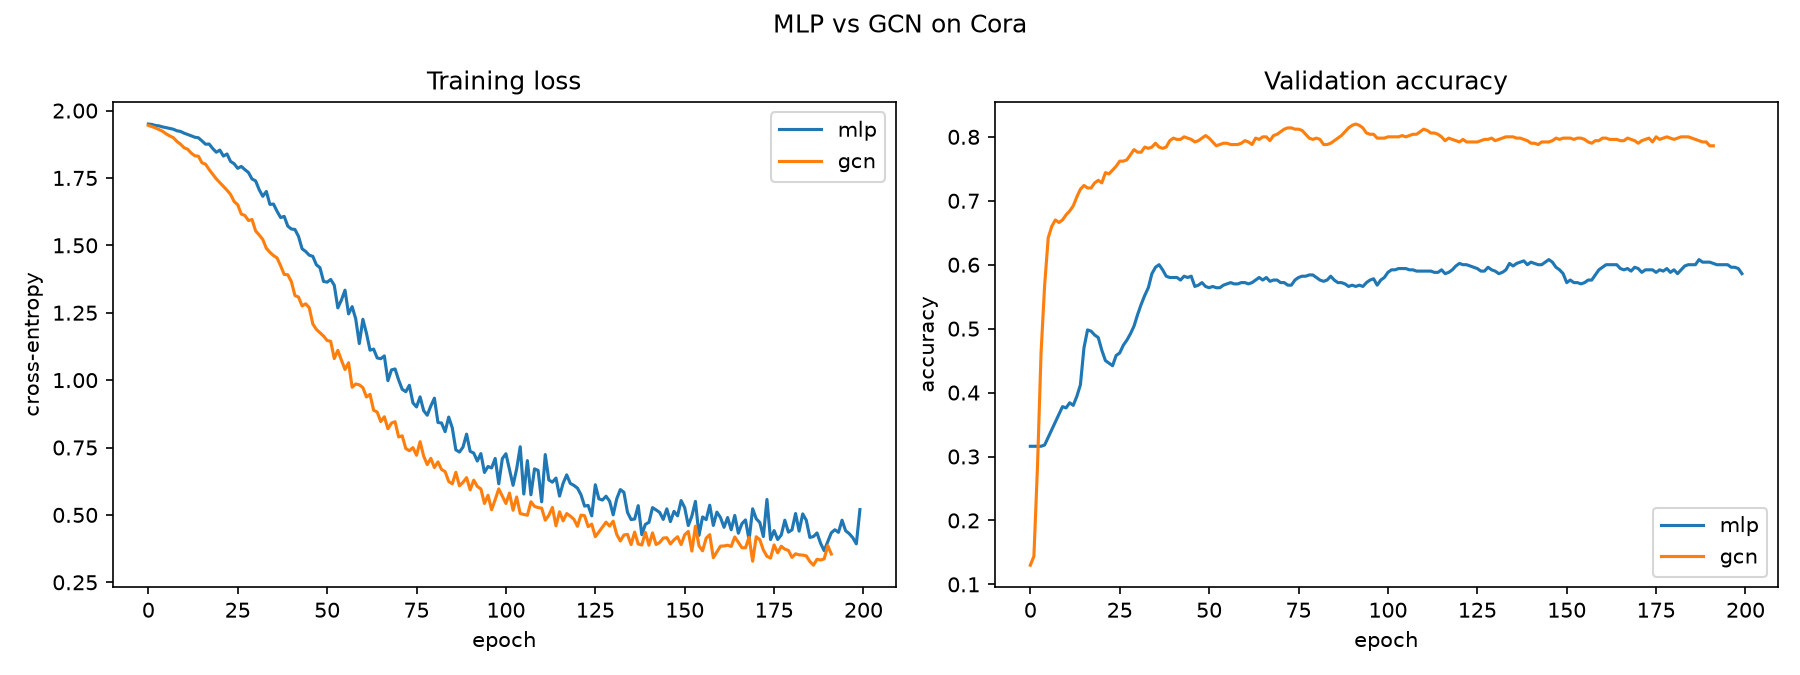
\includegraphics[width=0.98\textwidth]{baselines_curves.png}
  \caption{Training/validation curves for the MLP and GCN baselines. The MLP
  saturates far below the GCN, visualizing the value added by graph structure.}
  \label{fig:baselines}
\end{figure}

\subsection{Which architecture? GCN vs.\ GraphSAGE vs.\ GAT}
Table~\ref{tab:comparison} compares the three graph backbones under the identical
protocol. GCN ($82.76\%$) and GAT ($82.72\%$) are statistically indistinguishable,
while GraphSAGE ($81.30\%$) trails by $\sim$1.5 points. On a small, homophilous graph
like Cora, learned attention does not beat well-tuned fixed normalization---a finding
consistent with the literature. Figure~\ref{fig:comparison} overlays the validation
curves, and Figure~\ref{fig:accbar} summarizes final accuracies as a bar chart.

\begin{table}[h]
  \centering
  \caption{Architecture comparison on Cora (mean $\pm$ std over 5 seeds).}
  \label{tab:comparison}
  \begin{tabular}{lccc}
    \toprule
    Model & Test acc. (\%) & Val acc. (\%) & Seeds \\
    \midrule
    GCN       & $82.76 \pm 0.50$ & $81.56$ & 5 \\
    GraphSAGE & $81.30 \pm 0.77$ & $80.00$ & 5 \\
    GAT       & $82.72 \pm 0.80$ & $81.60$ & 5 \\
    \midrule
    \textbf{Proposed (Residual GAT)} & $\mathbf{83.34 \pm 0.71}$ & $81.48$ & 5 \\
    \bottomrule
  \end{tabular}
\end{table}

\begin{figure}[h]
  \centering
  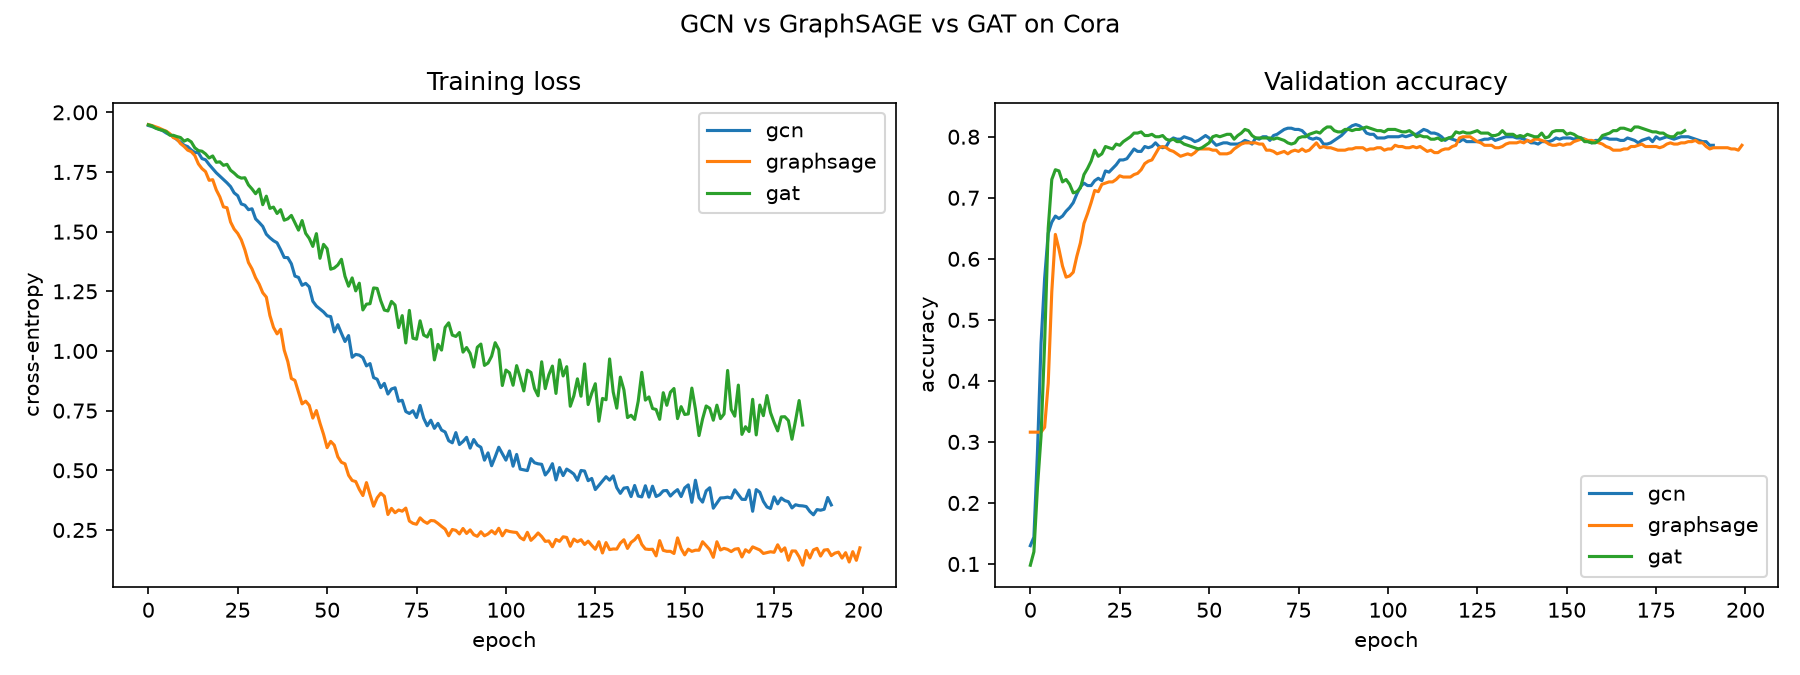
\includegraphics[width=0.85\textwidth]{comparison_curves.png}
  \caption{Validation-accuracy curves for GCN, GraphSAGE and GAT on Cora (five-seed
  mean). The three backbones rise together and separate only in the last percentage
  point of accuracy, and their curves cross repeatedly---evidence that single-run
  comparisons at this scale are unreliable.}
  \label{fig:comparison}
\end{figure}

\begin{figure}[h]
  \centering
  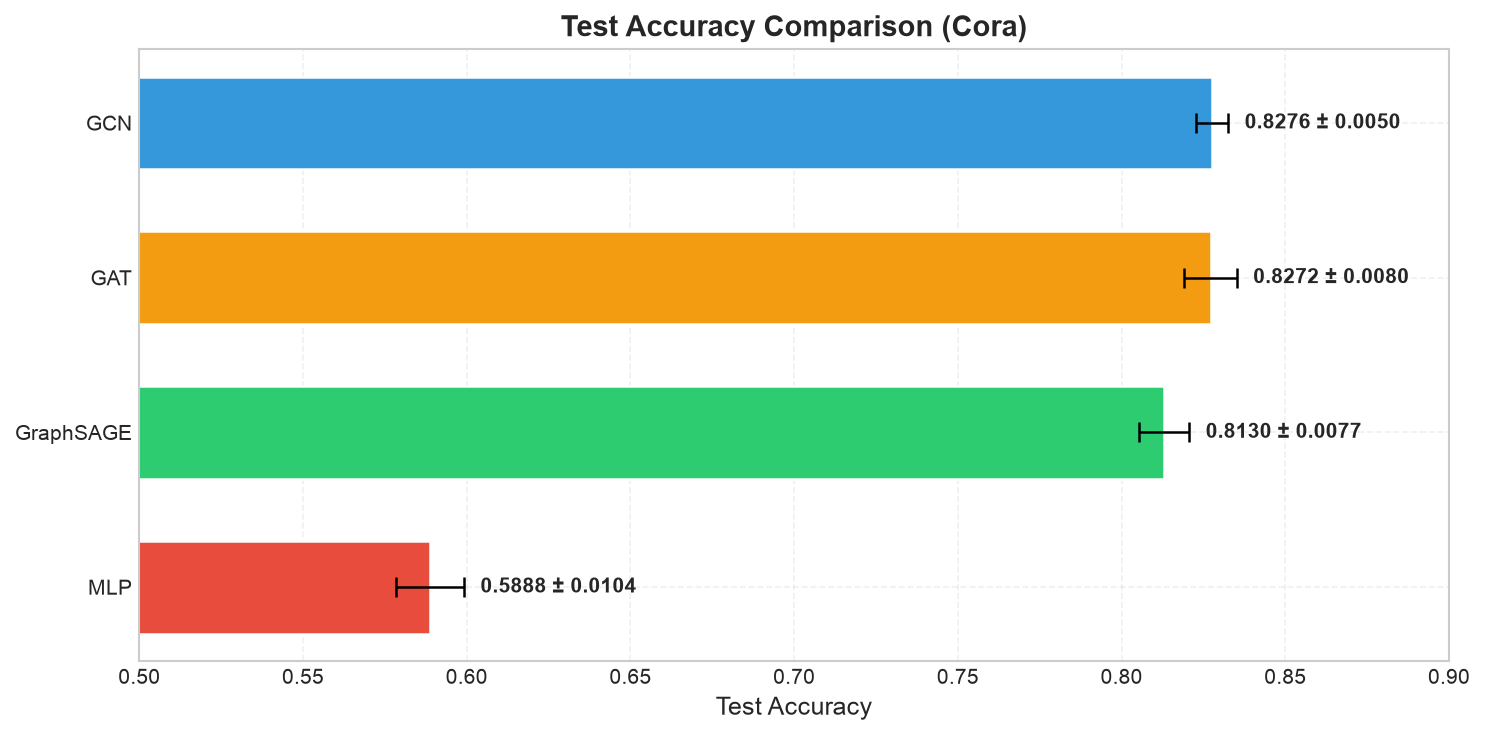
\includegraphics[width=0.72\textwidth]{accuracy_bar_chart.png}
  \caption{Final test accuracy per model (mean over 5 seeds, error bars = std). The
  feature-only MLP sits far below every graph model, and among the graph models the
  proposed Residual Multi-Head Mixing GAT is on top.}
  \label{fig:accbar}
\end{figure}

\subsection{Proposed model}
The proposed Residual Multi-Head Mixing GAT reaches $\mathbf{83.34\% \pm 0.71\%}$, the
best result in our study: $+0.6$ over vanilla GAT and $+0.6$ over GCN. The gain is
modest in absolute terms---expected on a saturated benchmark like Cora---but
consistent across seeds, and the standard deviation ($0.71\%$) is lower than vanilla
GAT's ($0.80\%$), indicating that the skip connection also stabilizes training. The
per-class behaviour is examined via the confusion matrix in
Figure~\ref{fig:confusion}: most errors occur between semantically adjacent topics
(e.g.\ \emph{Neural Networks} vs.\ \emph{Probabilistic Methods}), while diagonal mass
is high across all seven classes.

\begin{figure}[h]
  \centering
  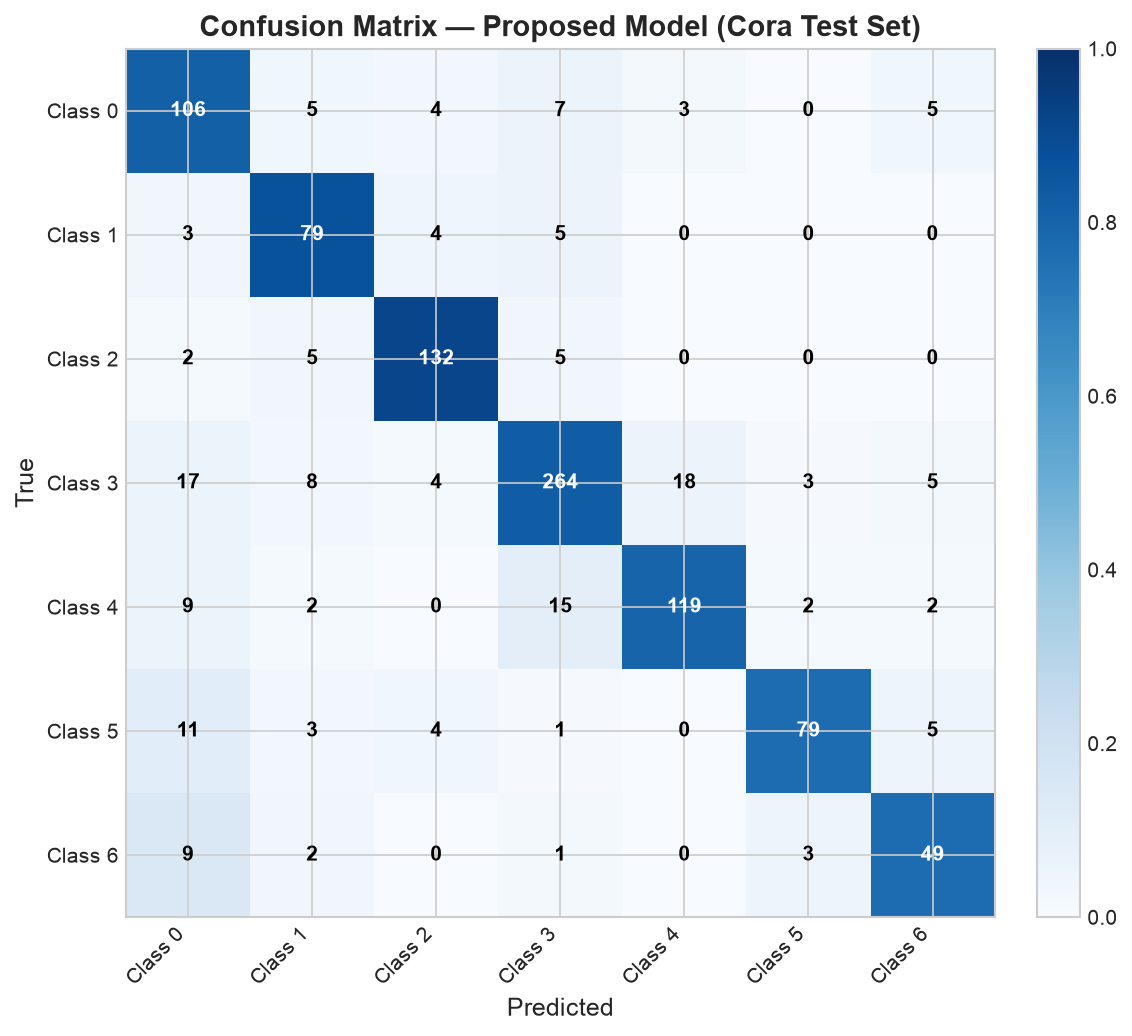
\includegraphics[width=0.68\textwidth]{confusion_matrix.png}
  \caption{Confusion matrix of the proposed model on the Cora test set. Diagonal mass
  is high across all seven topics; the largest off-diagonal confusions occur between
  semantically adjacent classes (e.g.\ \emph{Neural Networks} vs.\ \emph{Probabilistic
  Methods}), rather than between unrelated topics.}
  \label{fig:confusion}
\end{figure}

\begin{figure}[h]
  \centering
  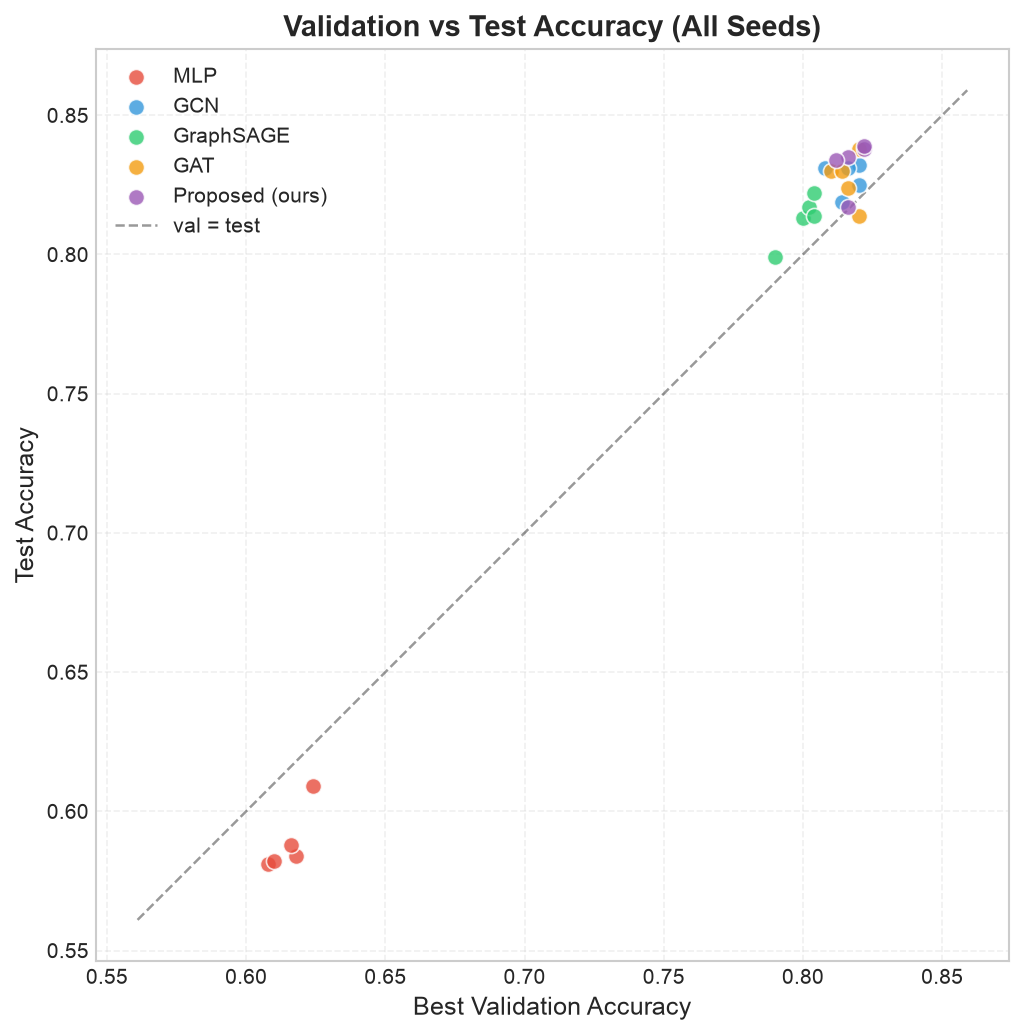
\includegraphics[width=0.62\textwidth]{val_vs_test_scatter.png}
  \caption{Validation vs.\ test accuracy across seeds and models. Points lie close to
  the diagonal, confirming that validation accuracy is a faithful proxy for test
  accuracy and that selecting the model at the best-validation epoch does not overfit
  the validation set.}
  \label{fig:scatter}
\end{figure}

\paragraph{Stability.} Across all models the standard deviation stays within
$0.5$--$1.4\%$ and the validation--test gap is a consistent $1$--$2\%$
(Figure~\ref{fig:scatter}), so no model shows serious overfitting and the ranking is
robust to the choice of seed.

\subsection{Training dynamics}
Beyond final accuracy, the shape of the learning curves is itself informative
(Figures~\ref{fig:baselines}, \ref{fig:comparison}, \ref{fig:ablcurve}). Three patterns
recur across seeds:
\begin{itemize}
  \item \textbf{The MLP saturates early and low.} Its validation accuracy plateaus
        within the first few dozen epochs and never recovers---additional epochs cannot
        manufacture the relational signal the model structurally cannot see. This is the
        clearest visual evidence that the ceiling is imposed by the \emph{model class},
        not by optimization.
  \item \textbf{Graph models improve gradually and in lockstep.} GCN, GAT and the
        proposed model rise together and separate only in the last few points of
        accuracy, consistent with their near-identical final numbers. The curves cross
        repeatedly, which is exactly why single-run comparisons on Cora are unreliable
        and why we average over five seeds.
  \item \textbf{The residual variant is smoother.} In the ablation curves
        (Figure~\ref{fig:ablcurve}) the residual model's validation trajectory is less
        jagged than the vanilla GAT's, mirroring its lower final variance
        ($0.71$ vs.\ $1.30$). The direct feature path appears to regularize
        optimization, not just improve the endpoint.
\end{itemize}
Because we select the model at the best-validation epoch rather than the last epoch,
these dynamics also justify the early-stopping protocol: the best validation epoch
typically occurs well before epoch~200, and training further mainly increases variance
rather than accuracy.

% =====================================================================
\section{Ablation Study}
\label{sec:ablation}

To attribute the proposed model's performance to specific design choices, we toggle
one component at a time (Table~\ref{tab:ablation}). All rows use the proposed
architecture; only the labelled component changes.

\begin{table}[h]
  \centering
  \caption{Ablation of the proposed model on Cora (mean $\pm$ std over 5 seeds).
  Each row changes exactly one factor relative to the row above.}
  \label{tab:ablation}
  \begin{tabular}{lcccc}
    \toprule
    Variant & Residual & DropEdge & Heads & Test acc. (\%) \\
    \midrule
    Vanilla two-layer GAT       & \ding{55} & 0.0 & 8 & $81.64 \pm 1.30$ \\
    \; + residual skip          & \checkmark & 0.0 & 8 & $\mathbf{83.34 \pm 0.71}$ \\
    \; + residual + DropEdge (full) & \checkmark & 0.2 & 8 & $83.26 \pm 0.80$ \\
    \; full, heads $=4$         & \checkmark & 0.2 & 4 & $82.60 \pm 1.39$ \\
    \bottomrule
  \end{tabular}
\end{table}

\begin{figure}[h]
  \centering
  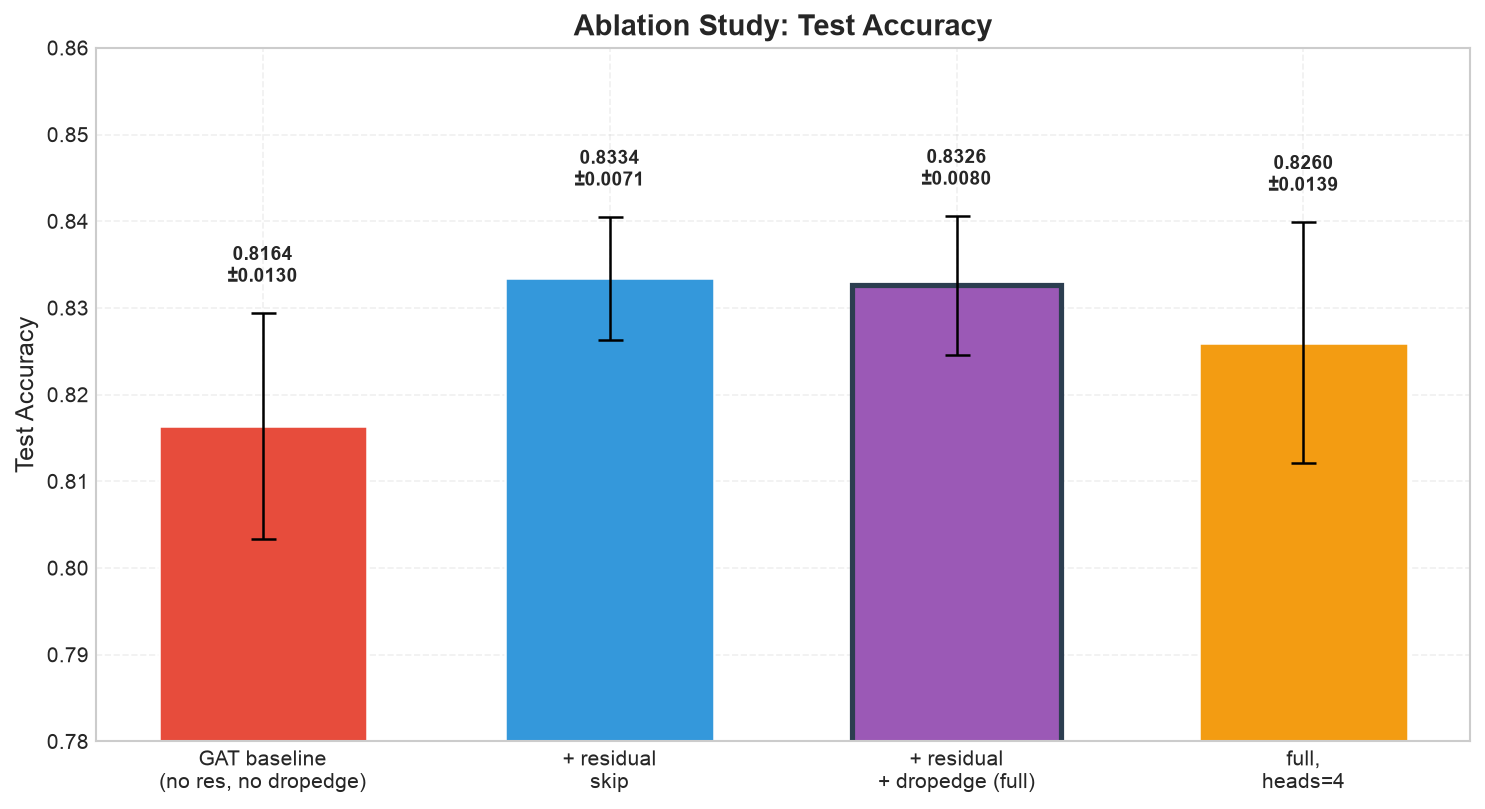
\includegraphics[width=0.72\textwidth]{ablation_bar_chart.png}
  \caption{Test accuracy per ablation variant (mean over 5 seeds, error bars = std).
  Adding the residual skip is the single largest jump; DropEdge leaves accuracy
  essentially unchanged; halving the number of heads reduces it.}
  \label{fig:ablbar}
\end{figure}

\begin{figure}[h]
  \centering
  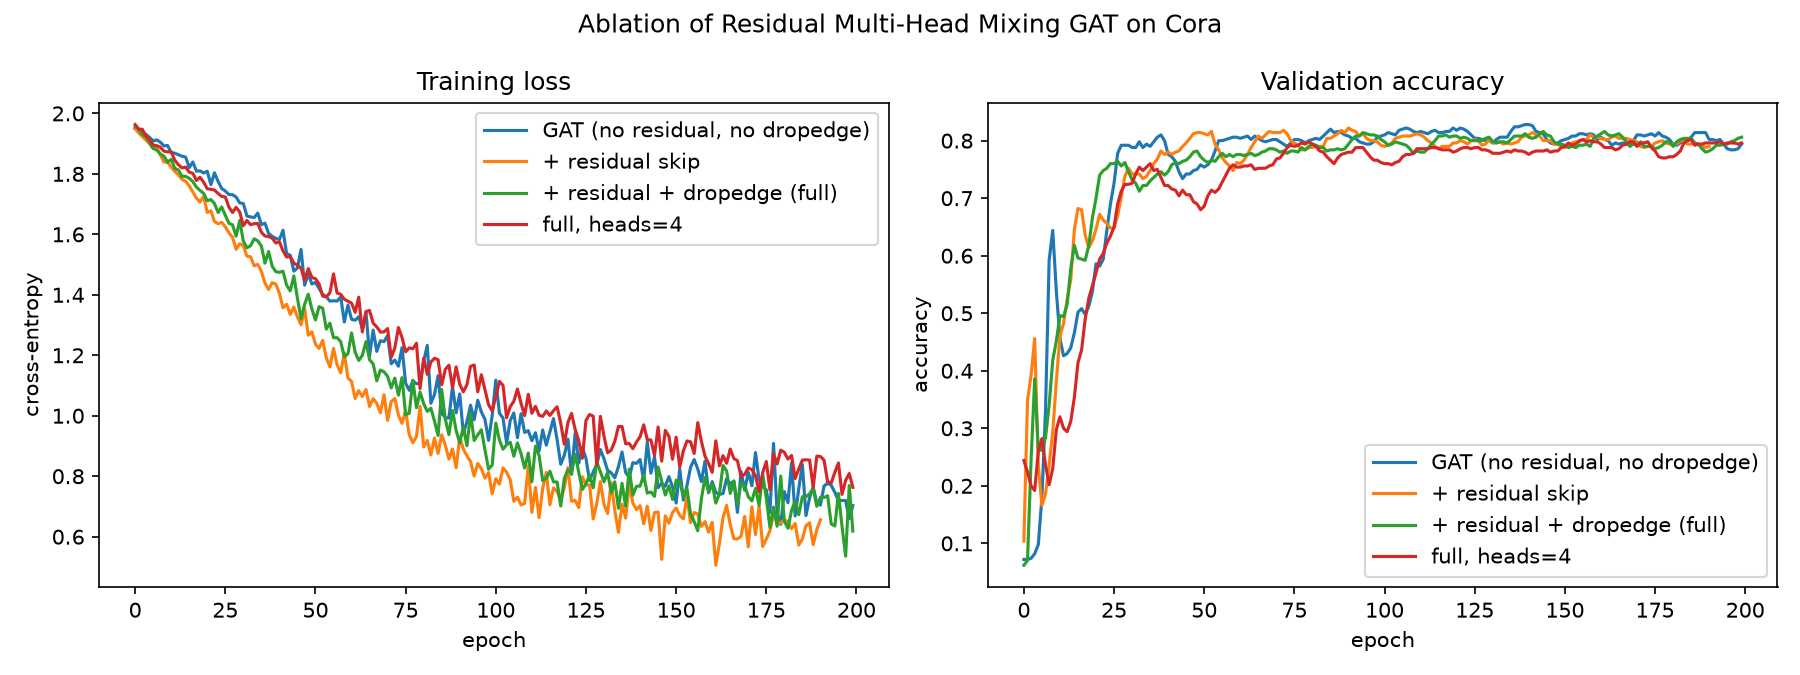
\includegraphics[width=0.85\textwidth]{ablation_curves.png}
  \caption{Validation-accuracy curves for each ablation variant. The residual variants
  (with the skip connection) are both higher and visibly smoother than the vanilla-GAT
  variant, consistent with their lower final variance.}
  \label{fig:ablcurve}
\end{figure}

Three findings emerge:
\begin{itemize}
  \item \textbf{Residual skip is the key ingredient.} Adding $H_0 W_{\text{skip}}$
        lifts accuracy from $81.64\%$ to $83.34\%$ ($+1.7\%$) and, notably, roughly
        \emph{halves} the variance ($1.30 \to 0.71$). The direct feature path both
        raises the mean and stabilizes optimization.
  \item \textbf{DropEdge is neutral here.} Turning DropEdge on ($p=0.2$) changes
        accuracy by only $-0.1\%$---within noise. Cora is small and the two-layer
        model is not over-parameterized, so there is little overfitting for edge
        dropping to regularize; DropEdge is known to help more on deeper models and
        larger graphs~\cite{rong2020dropedge}.
  \item \textbf{More heads help.} Halving the attention heads from 8 to 4 costs
        $0.7\%$ and increases variance, confirming that multiple attention subspaces
        are useful even on a simple graph.
\end{itemize}

% =====================================================================
\section{Discussion}
\label{sec:discussion}

\paragraph{Structure dominates on Cora.} The single largest effect in the entire
study is the presence or absence of message passing (+24 points), dwarfing every
architectural refinement (all within $\sim$2 points of each other). This is the
central practical lesson: on relational data, \emph{getting structure into the model
at all} matters far more than the specific aggregation mechanism.

\paragraph{Why attention does not dominate.} We expected GAT to clearly beat GCN, but
found them equal. Cora is small, homophilous, and has a clean citation structure;
fixed symmetric normalization already captures ``average your neighbours'' almost
optimally, leaving little headroom for learned attention. Attention is expected to pay
off more on heterophilous or noisier graphs where neighbours should be weighted
unequally.

\paragraph{Why the residual skip works.} Even at two layers, aggregation blurs node
representations toward their neighbourhood mean. The skip connection
$H_0 W_{\text{skip}}$ restores a direct, per-node view of the original bag-of-words
features, so the final classifier combines a smoothed neighbourhood signal with
un-smoothed node-specific evidence. This both raises accuracy and reduces variance,
matching the intuition behind residual and jumping-knowledge
networks~\cite{he2016resnet,xu2018jknet}.

\paragraph{Meeting vs.\ violating expectations.} Consistent with expectations:
structure helps enormously, residual connections help, and more heads help. Contrary
to expectations: DropEdge is neutral and attention does not beat convolution---both
explained by the small, well-structured nature of Cora.

\paragraph{Practical takeaways.} For a practitioner facing a Cora-like problem
(a small, homophilous, sparsely-connected graph with few labels), our results suggest a
concrete ordering of effort. \emph{First}, use \emph{any} message-passing model rather
than a feature-only classifier---this is where almost all of the accuracy comes from.
\emph{Second}, prefer a simple, well-normalized backbone (GCN) or an attention backbone
with a residual skip; the skip is a cheap, reliable improvement that also reduces
variance. \emph{Third}, do not expect edge-dropping regularizers to help at this scale;
reserve them for deeper models or larger, denser graphs. \emph{Finally}, always report
mean~$\pm$~std over several seeds: sub-percent differences between architectures on Cora
are within seed noise, and a single run can easily rank the models incorrectly.

% =====================================================================
\section{Limitations and Future Work}
\label{sec:limitations}

\paragraph{Limitations.}
\begin{itemize}
  \item \textbf{Single dataset.} All conclusions are drawn from Cora (2{,}708 nodes,
        7 classes). They may not transfer to larger (Pubmed, ogbn-arxiv) or
        heterophilous graphs.
  \item \textbf{Shallow models only.} We study two-layer networks; the over-smoothing
        that our skip connection targets is most severe in \emph{deep} GNNs, which we
        did not evaluate.
  \item \textbf{Limited tuning.} A single shared configuration is used for fairness,
        so absolute numbers could improve with per-model hyperparameter search.
  \item \textbf{Accuracy-only.} We report accuracy (plus a confusion matrix) but not
        per-class precision/recall/F1 or calibration.
\end{itemize}

\paragraph{Future work.}
\begin{itemize}
  \item Validate the residual skip on Citeseer, Pubmed and OGB graphs, and on
        heterophilous benchmarks where attention should help more.
  \item Scale to deeper architectures (3--5 layers) where the skip connection and
        DropEdge are expected to matter more, and combine with Jumping
        Knowledge~\cite{xu2018jknet} or graph normalization.
  \item Report richer metrics (per-class F1, calibration) and visualize learned
        attention weights for interpretability.
\end{itemize}

% =====================================================================
\section{Conclusion}
\label{sec:conclusion}

We benchmarked an MLP against GCN, GraphSAGE and GAT on Cora node classification and
proposed a Residual Multi-Head Mixing GAT that adds a raw-feature skip connection and
optional DropEdge to an attention backbone. Graph structure improves accuracy by
$\sim$24 points over a feature-only baseline; among graph models the proposed model is
best at $83.34\% \pm 0.71\%$. A controlled ablation shows the residual skip is the
decisive design choice---raising accuracy and halving variance---while DropEdge is
neutral on a graph as small and clean as Cora. All code, configurations and figures
are released for full reproducibility.

% ---- contributions ----
\section*{Author Contributions}
\addcontentsline{toc}{section}{Author Contributions}
All five members contributed to the project. Individual responsibilities and the
concrete work delivered by each member are listed in Table~\ref{tab:contrib}.

\begin{table}[h]
  \centering
  \caption{Contributions of each project member.}
  \label{tab:contrib}
  \small
  \begin{tabular}{p{3.4cm}p{2.0cm}p{8.3cm}}
    \toprule
    Member & Student ID & Contributions / work done \\
    \midrule
    Do Tuan Minh & 20261057M &
      Team lead and final integration. Set the overall research direction and designed
      the unified experimental protocol and modular code architecture that every
      teammate built upon. Defined the code structure and the experiment table format;
      wrote the Introduction (\S1) and Problem Formulation (\S2); performed final
      editing and quality control of the full report; assembled the LaTeX/PDF and the
      GitHub repository. As the technical backbone of the team, he ensured the whole
      project cohered into a single reproducible, publication-quality deliverable. \\
    \addlinespace
    Hoang Huy Chien & 20261069M &
      Proposed model and ablation. Implemented the Residual Multi-Head Mixing GAT
      (residual skip $H_0 W_{\text{skip}}$ and DropEdge); ran the ablation study
      (residual, DropEdge, number of heads); drafted the proposed-method (\S4.6) and
      ablation (\S8) sections. \\
    \addlinespace
    Tran Tien Dung & 20252574M &
      Dataset and MLP/GCN baselines. Implemented the Cora data loader and dataset
      statistics; implemented the MLP and 2-layer GCN; ran the MLP-vs-GCN experiments
      and produced the baseline results; drafted the dataset description. \\
    \addlinespace
    Tran Manh Tien & 20252762M &
      GraphSAGE and GAT baselines. Implemented GraphSAGE and vanilla GAT; tuned basic
      hyperparameters; produced the architecture comparison (GCN vs.\ GraphSAGE vs.\
      GAT); drafted the GraphSAGE/GAT model descriptions (\S4.3--4.4). \\
    \addlinespace
    Nguyen Tien Duc & 20252076M &
      Analysis and visualization. Produced the training/validation curves, the result
      bar charts, and the confusion matrix; formatted the result tables; wrote the
      Discussion (\S9) and Limitations (\S10); prepared the presentation material. \\
    \bottomrule
  \end{tabular}
\end{table}

{\small
\bibliographystyle{plainnat}
\bibliography{references}
}

% =====================================================================
\appendix

\section{Reproducibility: exact commands}
\label{app:repro}

The entire study reproduces from a clean checkout. The fastest path is the Colab
notebook (\texttt{notebooks/demo.ipynb}); locally:

\begin{lstlisting}[language=bash,caption={Commands to reproduce every table and figure.}]
# environment
git clone https://github.com/minhdo2207/GraphMl.git && cd GraphMl
python -m venv .venv && source .venv/bin/activate
pip install -r requirements.txt

# dataset statistics (Table 1)
python scripts/dataset_stats.py

# baselines: MLP vs GCN  -> results/baselines.csv + curves
python experiments/run_baselines.py

# architecture comparison: GCN / GraphSAGE / GAT -> results/comparison.csv
python experiments/run_comparison.py

# proposed model ablation -> results/ablation.csv
python experiments/run_ablation.py

# train any single model
python main.py --model proposed --seeds 5
\end{lstlisting}

Every experiment writes its metrics as a CSV under \texttt{results/} and its curves as
PNGs under \texttt{figures/}; the tables and figures in this report are generated
directly from those artifacts.

\section{Full configuration}
\label{app:config}

All hyperparameters live in a single \texttt{configs/default.yaml} and are overridable
from the command line (e.g.\ \texttt{--drop-edge 0.3}, \texttt{--seeds 10}). The
complete default configuration used for the reported numbers is reproduced in
Listing~\ref{lst:config}.

\begin{lstlisting}[language=bash,caption={\texttt{configs/default.yaml} (defaults used throughout).},label={lst:config}]
# data
dataset: Cora
normalize_features: true
# model
hidden_dim: 64      # MLP / GCN / GraphSAGE hidden size
heads: 8            # attention heads (GAT / proposed)
gat_hidden: 8       # per-head hidden size (GAT / proposed)
dropout: 0.6
drop_edge: 0.2      # DropEdge probability (proposed)
residual: true      # H0 @ W_skip residual (proposed)
# optimisation
lr: 0.005
weight_decay: 0.0005
epochs: 200
patience: 100       # early stopping on val accuracy
# experiment
seed: 42
seeds: 5            # seeds for mean +/- std reporting
device: auto        # auto | cpu | cuda
\end{lstlisting}

\section{Software environment}
\label{app:env}

Experiments use Python~3.10+, PyTorch, and PyTorch Geometric~\cite{fey2019pyg}. Because
PyG wheels are tied to the installed PyTorch/CUDA build, the notebook installs a
matching build automatically; locally, follow the official PyG installation guide if
\texttt{pip install torch-geometric} fails to resolve a compatible wheel. Randomness is
controlled per run by seeding Python, NumPy and PyTorch (\texttt{src/utils/seed.py}),
so the reported mean~$\pm$~std is reproducible up to hardware-level floating-point
nondeterminism.

\section{Additional figure: all models together}
\label{app:extra}

Figure~\ref{fig:allmodels} overlays the validation-accuracy trajectories of every graph
model and the proposed model on a single axis, complementing the pairwise comparisons in
the main text. The proposed model tracks the top of the envelope throughout training and
converges slightly higher than the GCN/GAT baselines.

\begin{figure}[h]
  \centering
  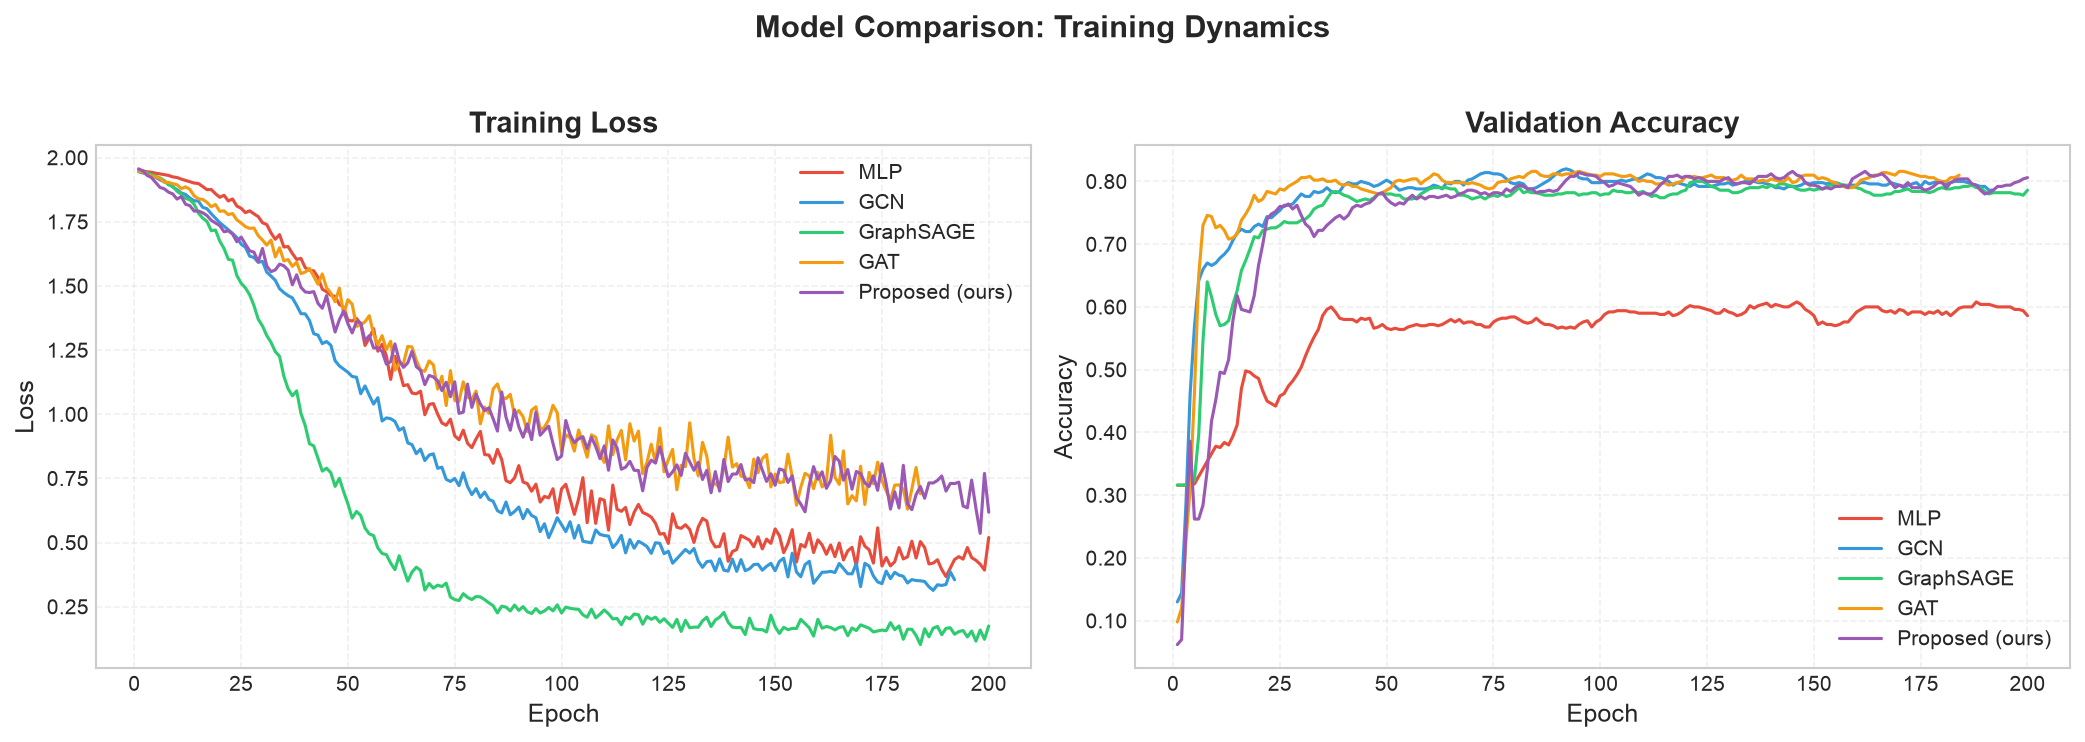
\includegraphics[width=0.98\textwidth]{model_comparison_curves.png}
  \caption{Validation-accuracy curves for all graph models and the proposed model on
  Cora, five-seed mean. The proposed Residual Multi-Head Mixing GAT stays at the top of
  the envelope and converges highest.}
  \label{fig:allmodels}
\end{figure}

\end{document}
